\begin{figure}[ht!]
        \centering
        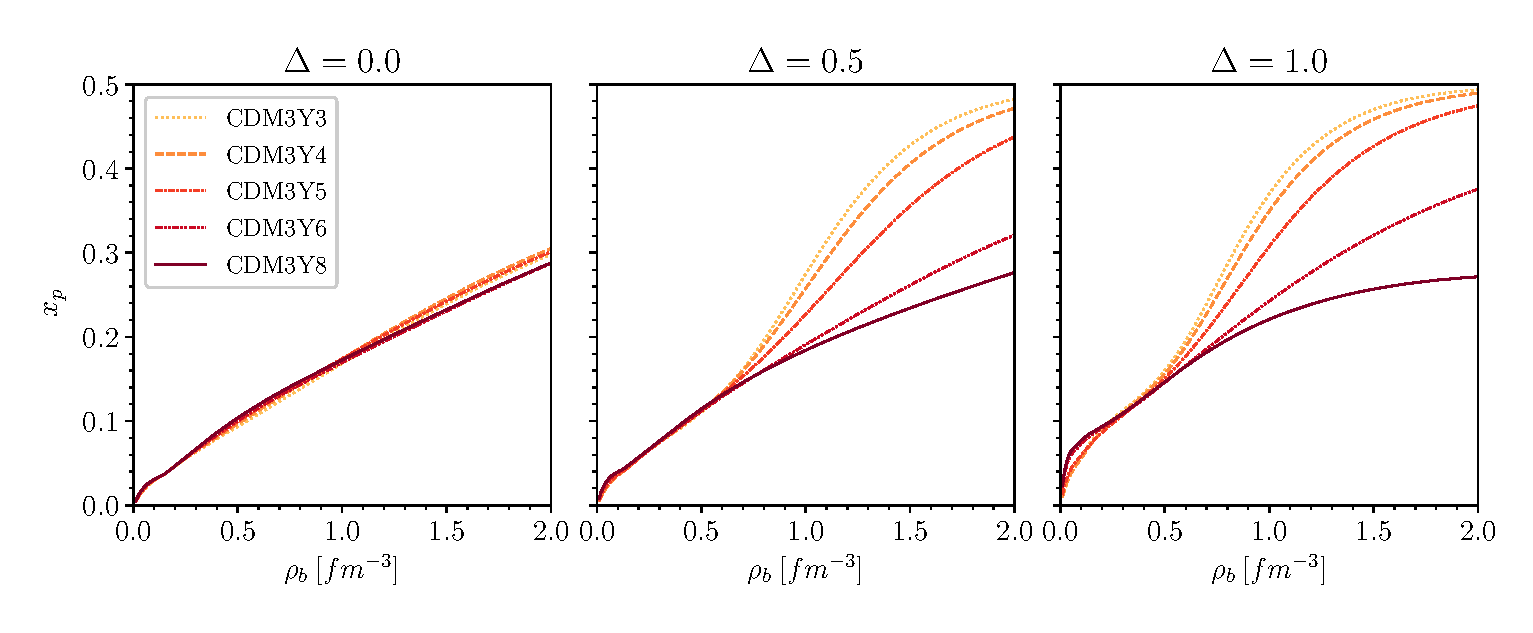
\includegraphics[width=\textwidth]{fig/xp.eps}
        \caption{Proton fraction $x_p$ of \textbeta-stable \gls{NM} at different baryon density and spin polarity for CDM3Y$n$ interactions.}
        \label{fig:xp}
\end{figure} 
\begin{figure}[ht!]
        \centering
        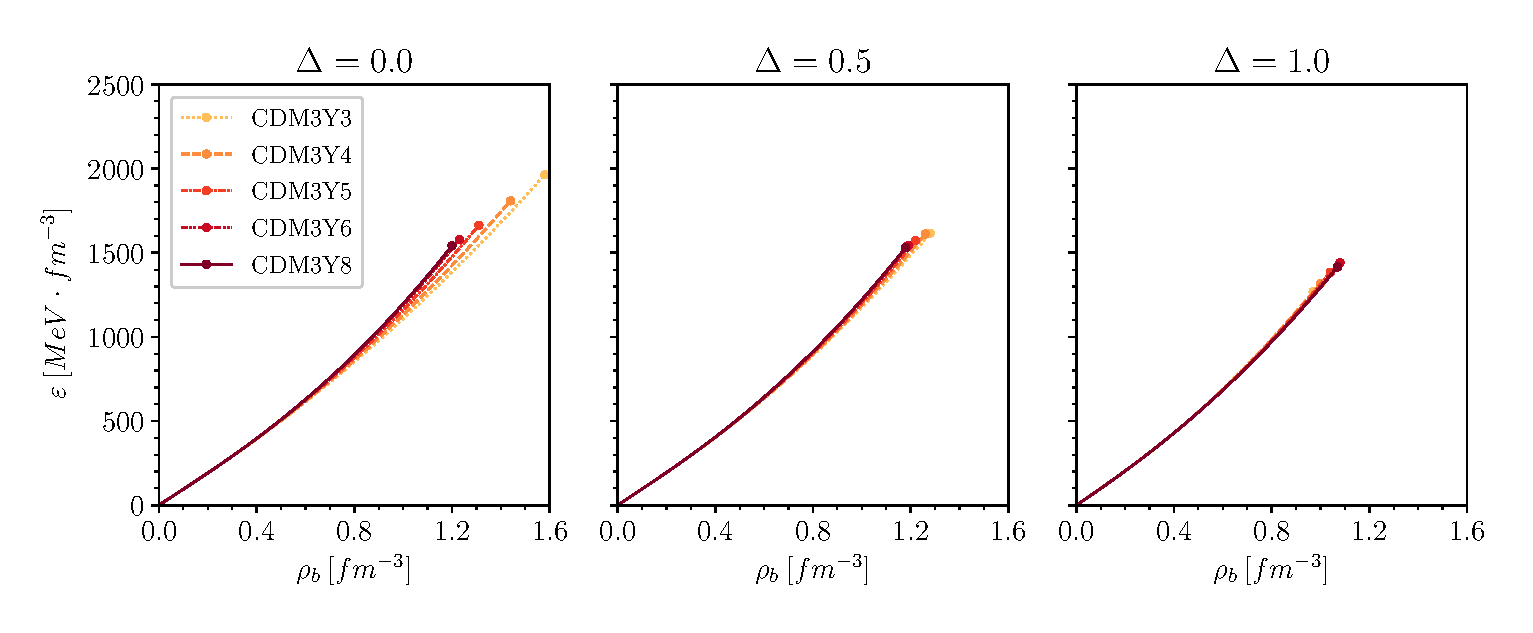
\includegraphics[width=\textwidth]{fig/E.eps}
        \caption{Total mass-energy density of \textbeta-stable \gls{NM} at varying spin polarity with different interaction models.}
        \label{fig:e}
\end{figure} 
\begin{figure}[ht!]
        \centering
        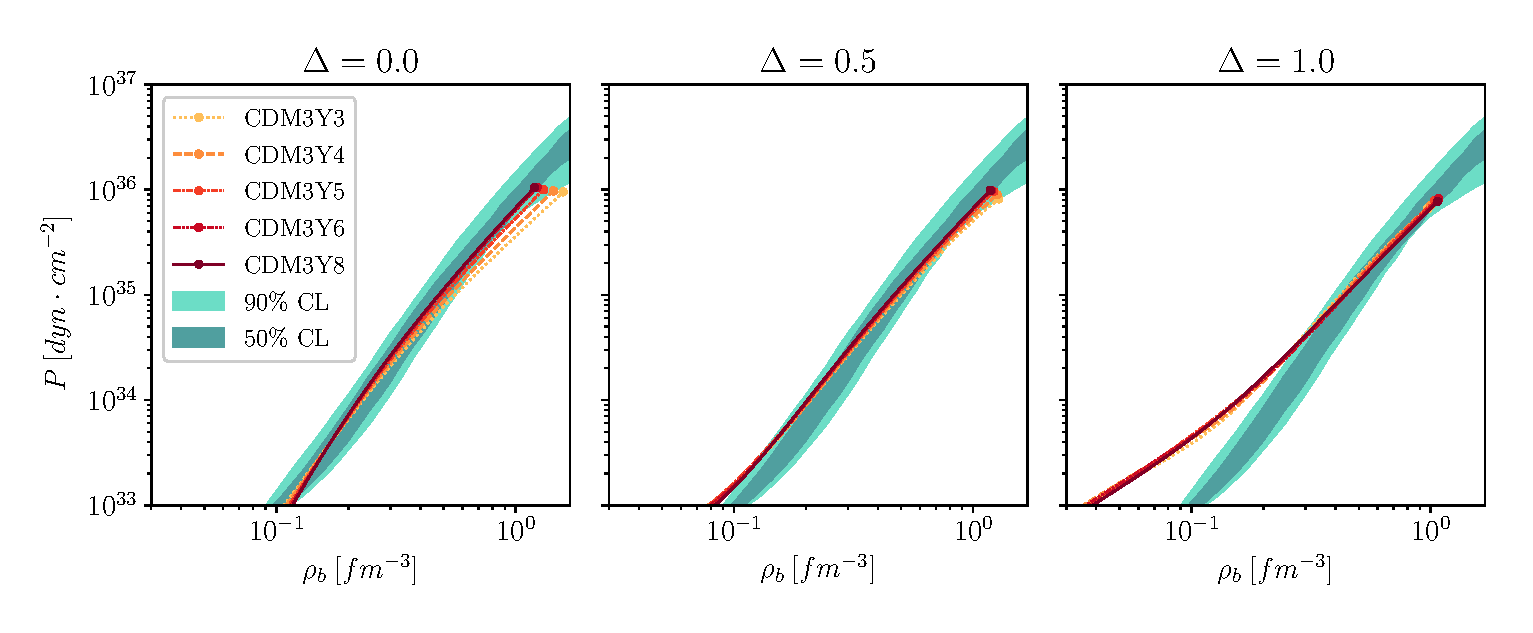
\includegraphics[width=\textwidth]{fig/P.eps}
        \caption{Total pressure of \textbeta-stable \gls{NM} at several values of $\Delta$ with different CDM3Y$n$ models.}
        \label{fig:p}
\end{figure} 
\begin{figure}[ht!]
        \centering
        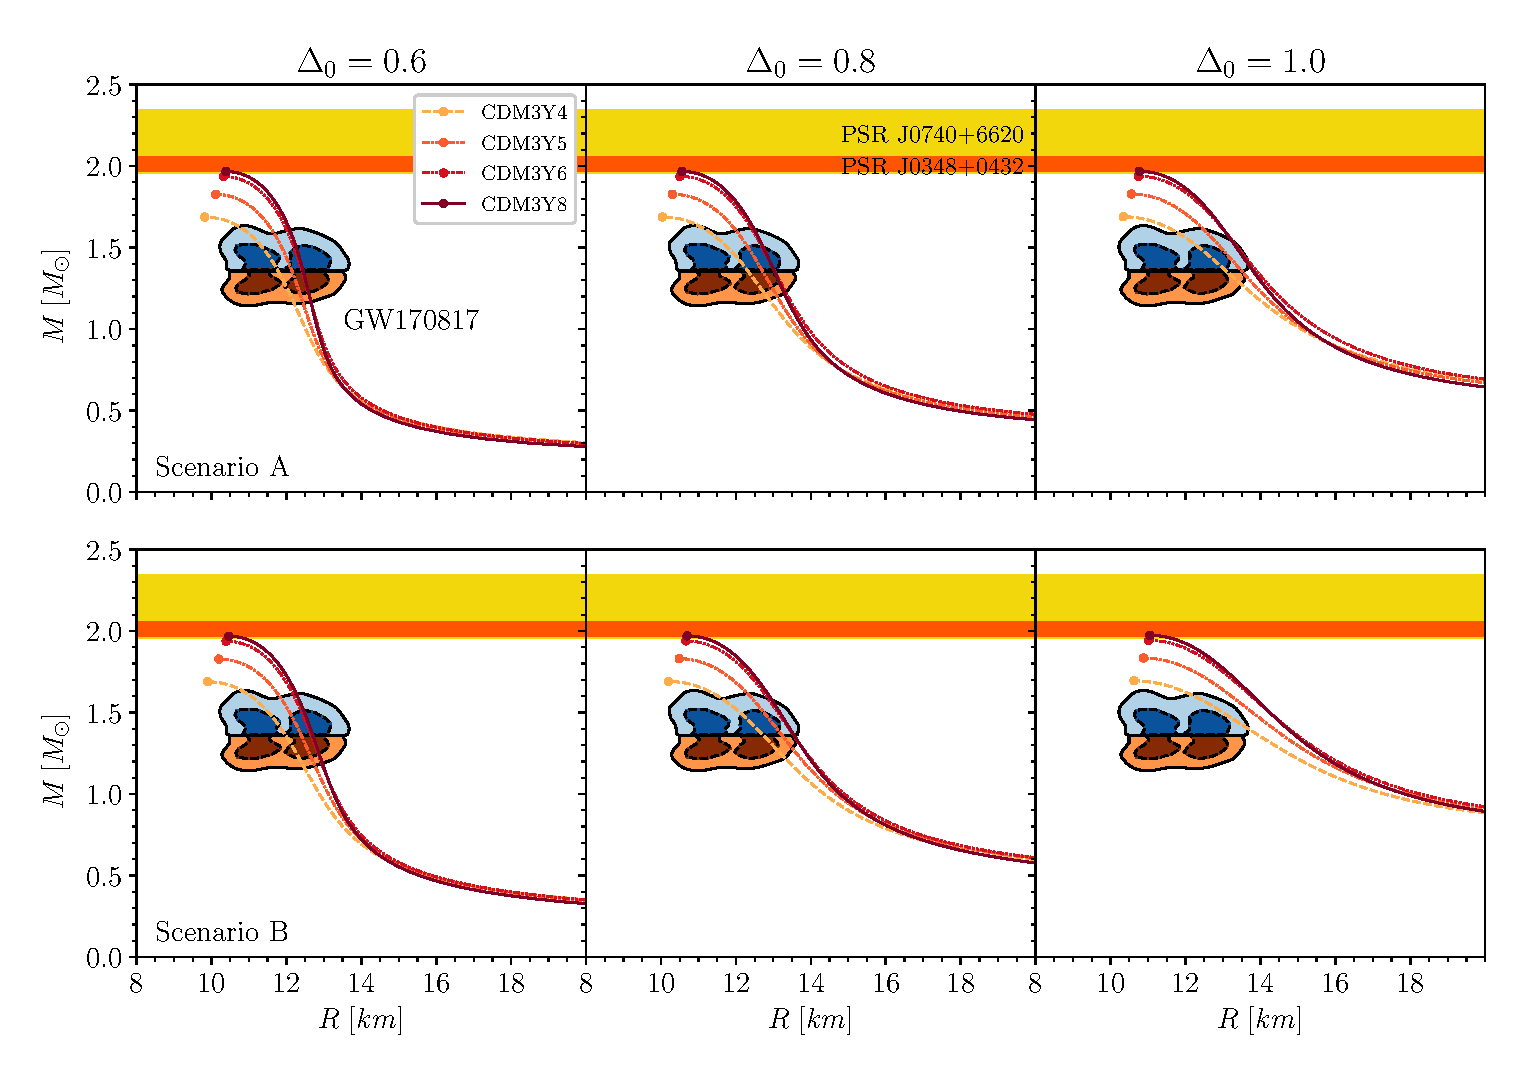
\includegraphics[width=\textwidth]{fig/MR.eps}
        \caption{The relation between gravitational mass $M$ and the radius $R$ of the \gls{NS} according to the corresponding model and polarity.}
        \label{fig:mr}
\end{figure} 
\begin{figure}[ht!]
        \centering
        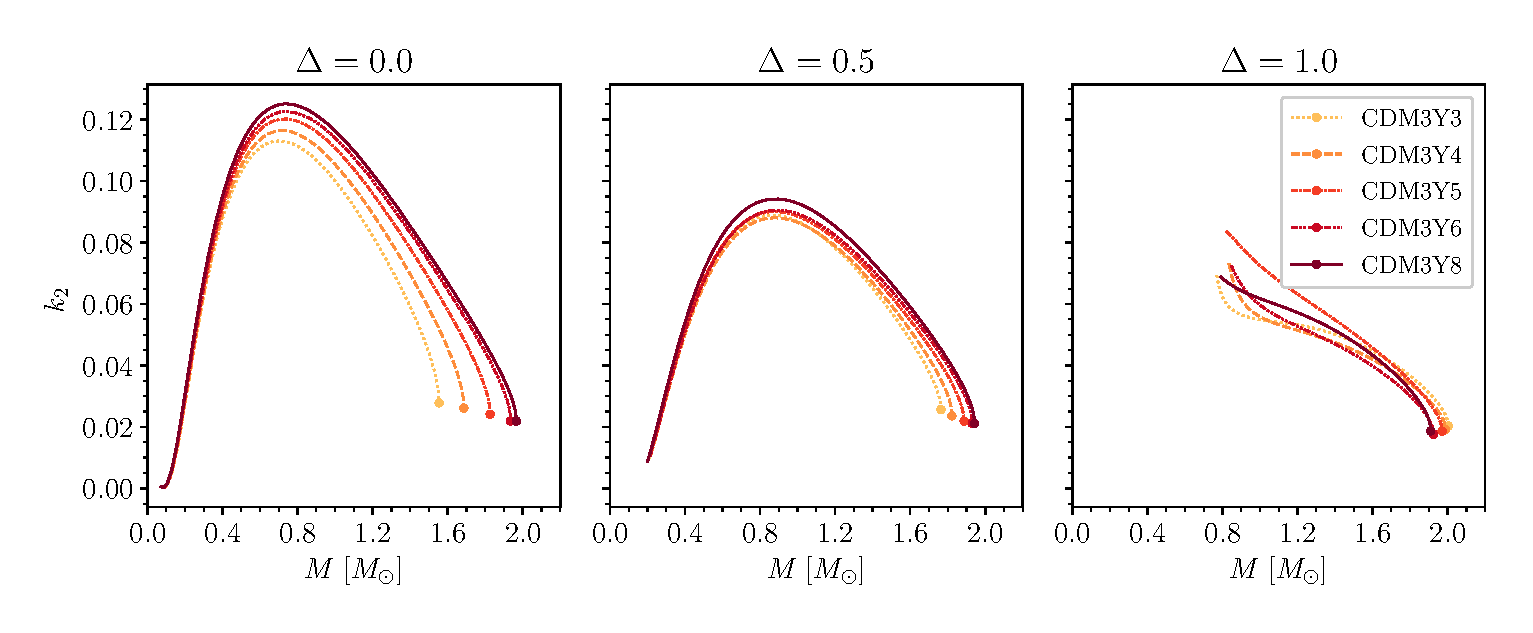
\includegraphics[width=\textwidth]{fig/k2.eps}
        \caption{\gls{GE} tidal Love number at 2\textsuperscript{nd} order $k_2$ as function of \gls{NS} mass computed with CDM3Y$n$ models at different spin polarities.}
        \label{fig:k2}
\end{figure} 
\begin{figure}[ht!]
        \centering
        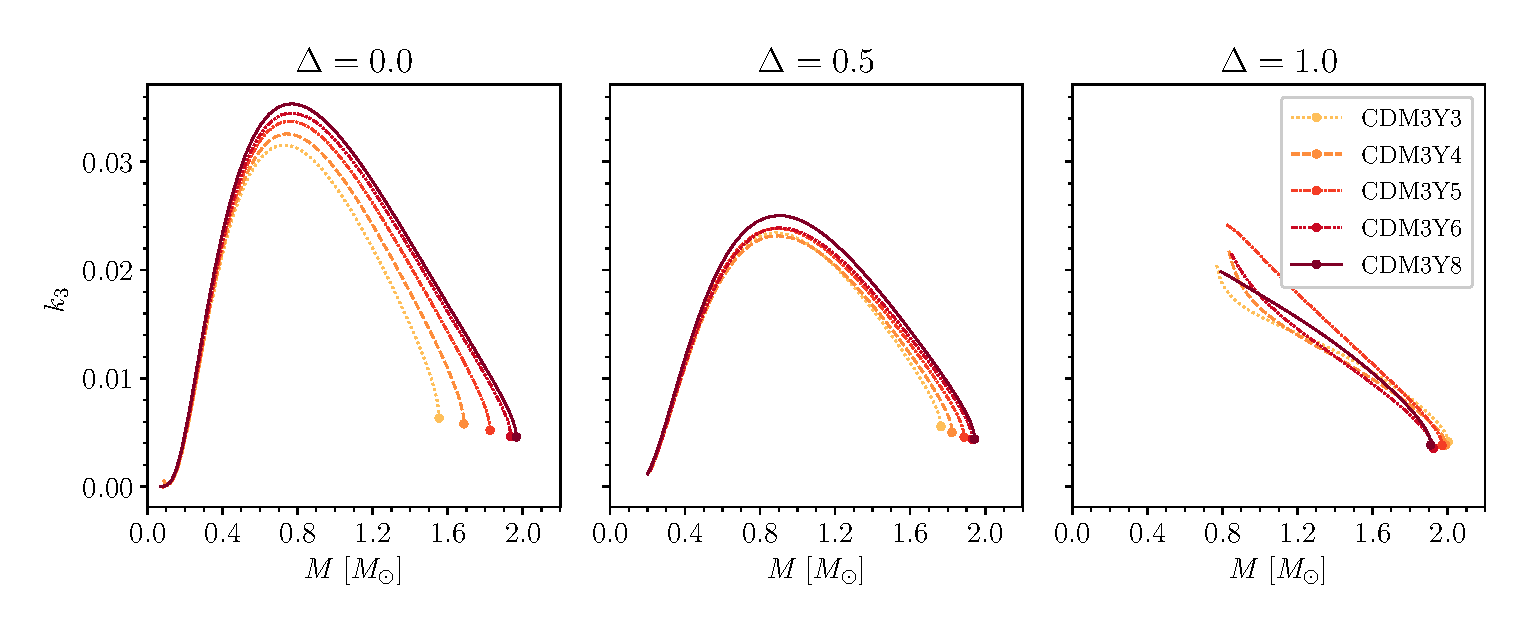
\includegraphics[width=\textwidth]{fig/k3.eps}
        \caption{Same as Figure \ref{fig:k2} for $k_3$.}
        \label{fig:k3}
\end{figure} 
\begin{figure}[ht!]
        \centering
        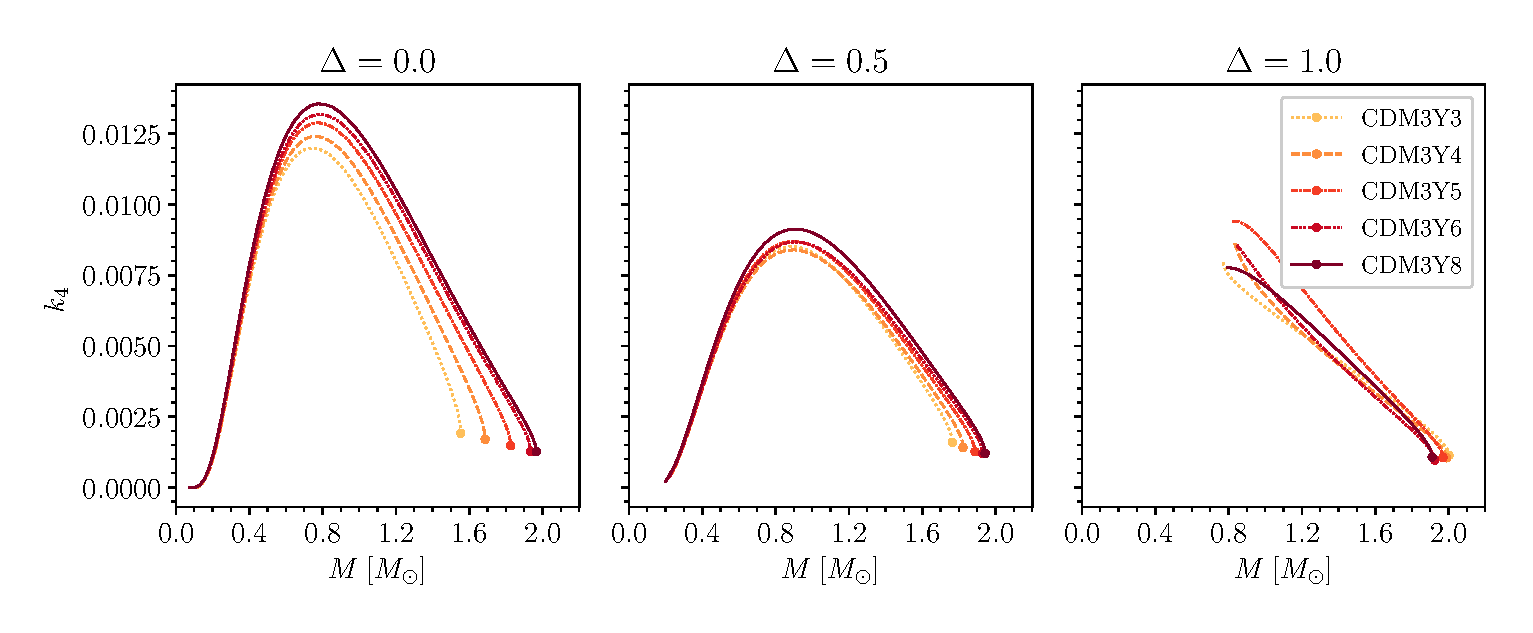
\includegraphics[width=\textwidth]{fig/k4.eps}
        \caption{Same as Figure \ref{fig:k2} for $k_4$.}
        \label{fig:k4}
\end{figure} 
\begin{figure}[ht!]
        \centering
        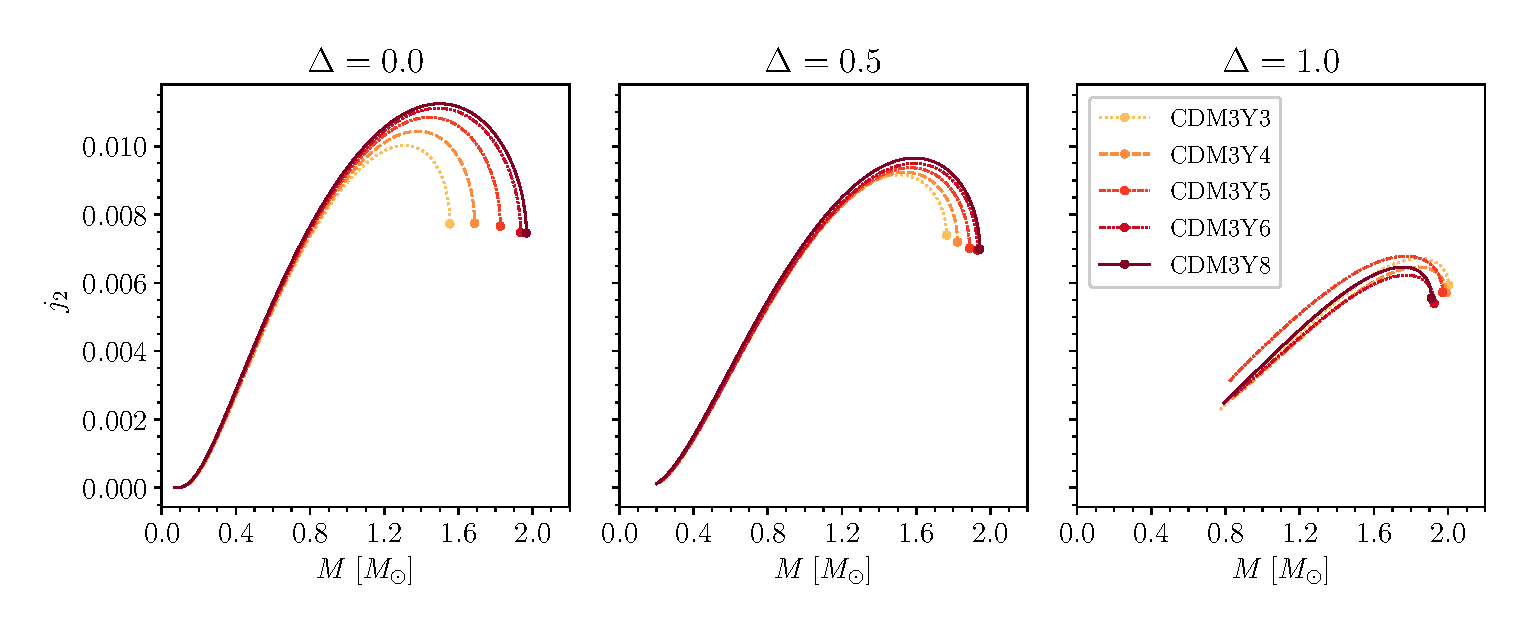
\includegraphics[width=\textwidth]{fig/j2_stat.eps}
        \caption{\gls{GM} tidal Love number at 2\textsuperscript{nd} order $j_2$ as function of \gls{NS} mass computed with CDM3Y$n$ models of \emph{strictly static fluid} at different polarities.}
        \label{fig:j2_stat}
\end{figure} 
\begin{figure}[ht!]
        \centering
        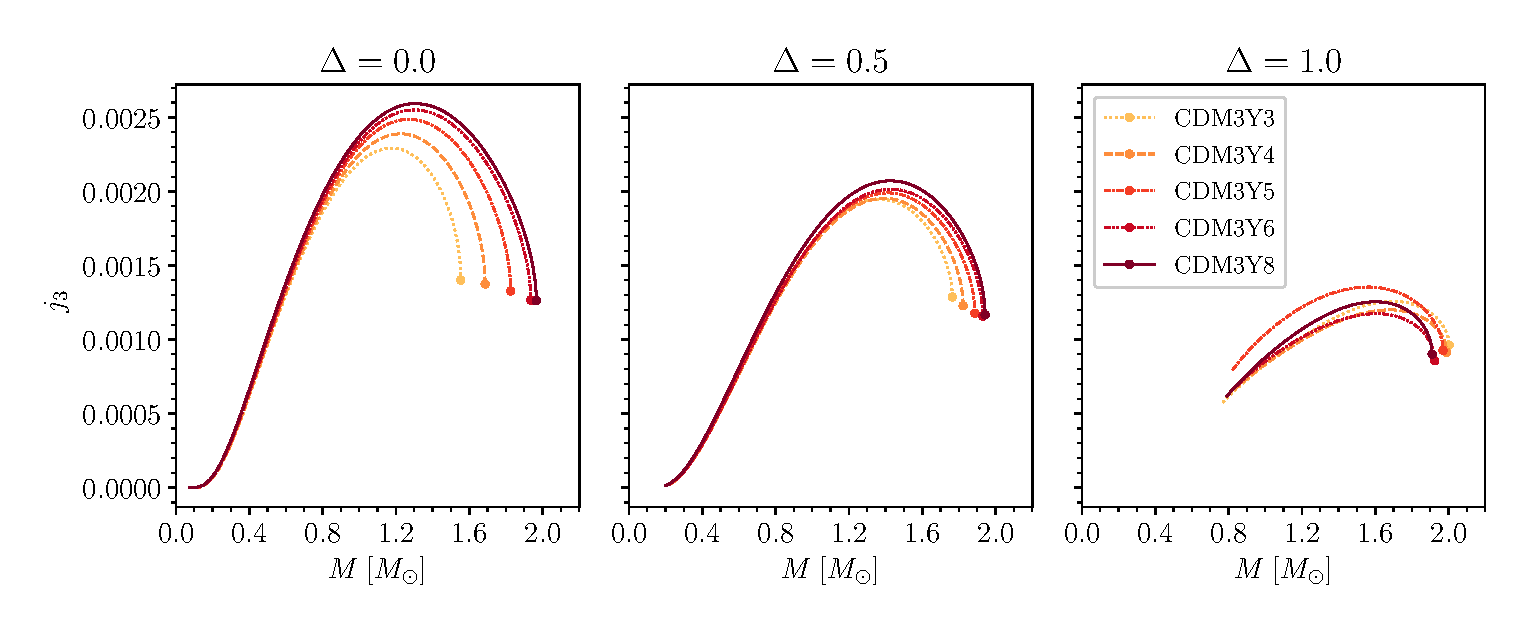
\includegraphics[width=\textwidth]{fig/j3_stat.eps}
        \caption{Same as Figure \ref{fig:j2_stat} for $j_3$.}
        \label{fig:j3_stat}
\end{figure} 
\begin{figure}[ht!]
        \centering
        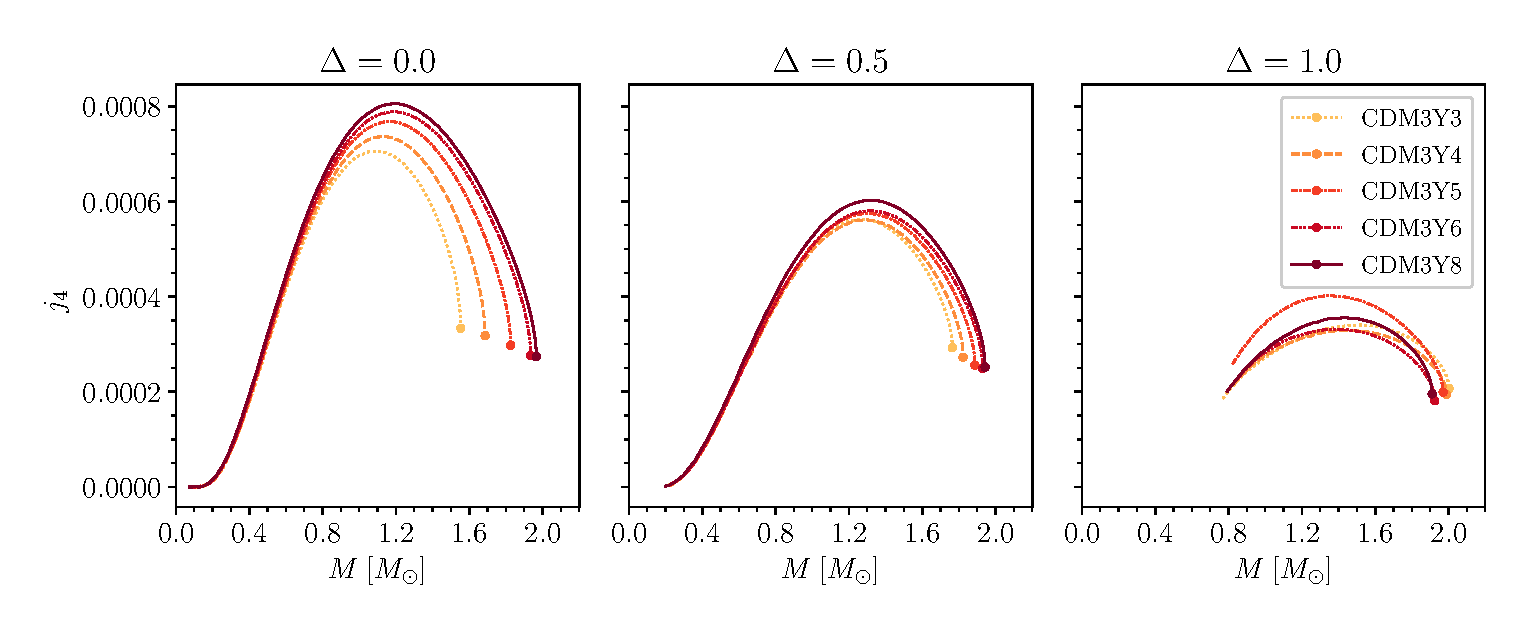
\includegraphics[width=\textwidth]{fig/j4_stat.eps}
        \caption{Same as Figure \ref{fig:j2_stat} for $j_4$.}
        \label{fig:j4_stat}
\end{figure} 
\begin{figure}[ht!]
        \centering
        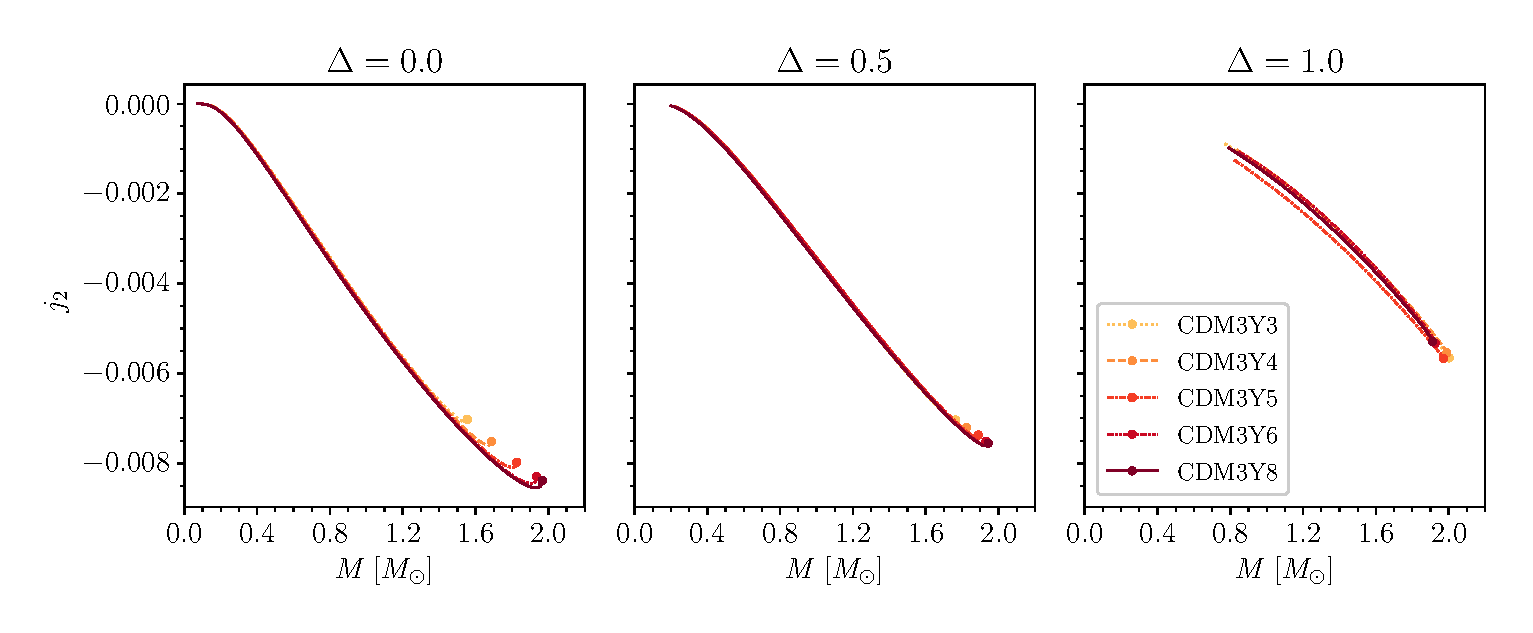
\includegraphics[width=\textwidth]{fig/j2_irrot.eps}
        \caption{\gls{GM} tidal Love number at 2\textsuperscript{nd} order $j_2$ as function of \gls{NS} mass computed with CDM3Y$n$ models of \emph{irrotational fluid} at different polarities.}
        \label{fig:j2_irrot}
\end{figure} 
\begin{figure}[ht!]
        \centering
        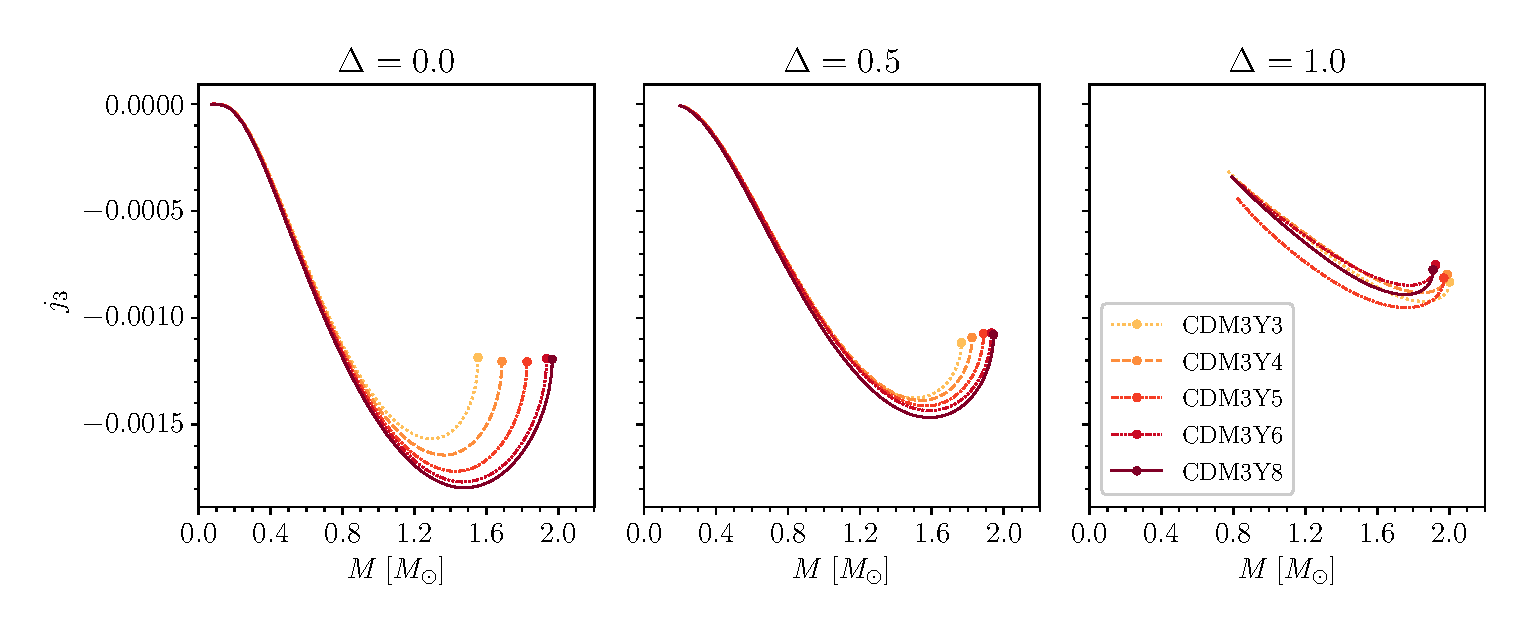
\includegraphics[width=\textwidth]{fig/j3_irrot.eps}
        \caption{Same as Figure \ref{fig:j2_irrot} for $j_3$.}
        \label{fig:j3_irrot}
\end{figure} 
\begin{figure}[ht!]
        \centering
        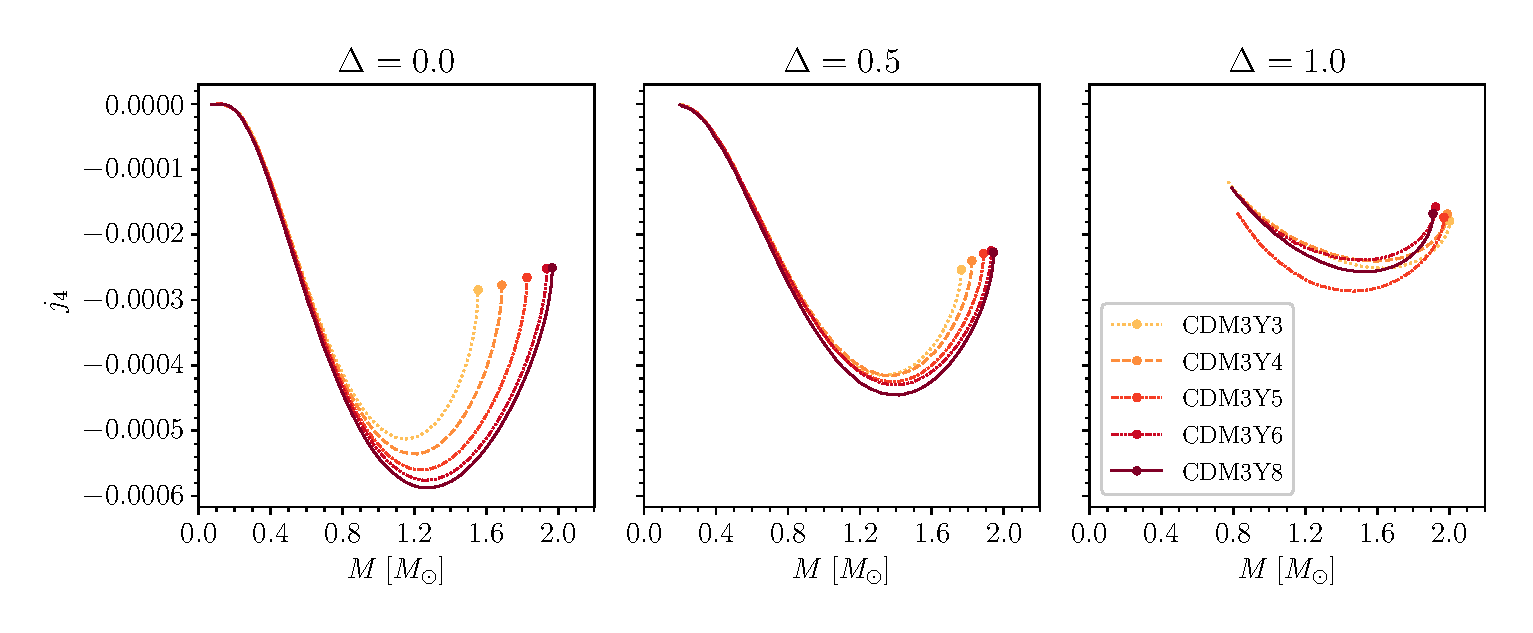
\includegraphics[width=\textwidth]{fig/j4_irrot.eps}
        \caption{Same as Figure \ref{fig:j2_irrot} for $j_4$.}
        \label{fig:j4_irrot}
\end{figure} 
